\thispagestyle{empty}

\lhead[\small\thepage]{\small\em An Invaluable Contribution}

\begin{figure}[h]
\centering
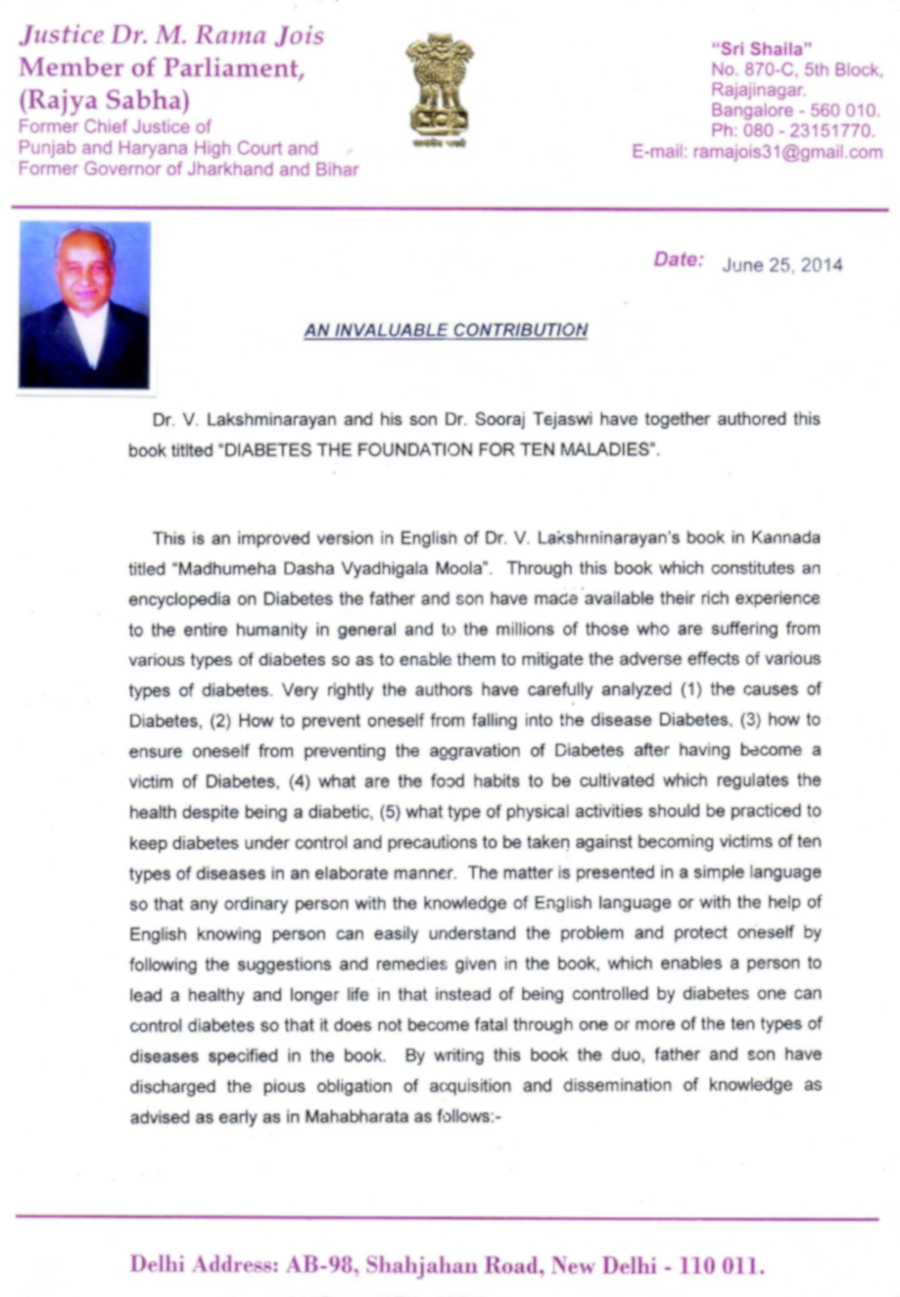
\includegraphics[scale=2.1]{images/002.jpg}
\end{figure}

\newpage

\begin{center}
\textbf{:: 2 ::}
\end{center}

\begin{figure}[h]
\centering
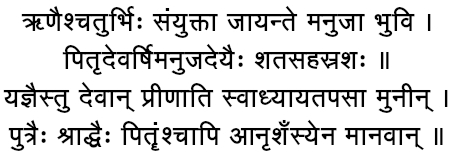
\includegraphics[scale=2.5]{images/002a.jpg}
\end{figure}

ॠणैश्चतुर्भिः संयुक्ता जायन्ते मानवा भुवि ।
पितृदेवर्षिमनुजैर्देयं तेभ्यश्र धर्मतः ॥
यज्ञैस्तु देवान् प्रीणाति स्वाध्यायतपसा मुनीन् ।
पुत्रैः श्राद्धैः पितॄंश्चापि आनृशंस्येन मानवान् ॥

\begin{quote}
\textit{\textbf{Every individual should discharge four pious obligations. They are Devaruna (towards God), Pitruruna (towards parents), Rishiruna (towards teachers) and Manavaruna (towards humanity).}}

\textit{\textbf{A man should discharge Pitruruna by maintaining continuity of the family, Devaruna by worship of God, Rishiruna by the acquisition and dissemination of knowledge, and Manavaruna by every type of social service. [Mahabharata, Adiparva, Ch-119, 17 \& 19].}}
\end{quote}

I say without any hesitation that father and son have ably discharged everyone of the four pious obligations as required in Mahabharata and in particular the third namely acquisition and dissemination of knowledge and also the fourth debt due to humanity.

I pray Almighty to enable them to serve humanity throughout their life time contributing such useful knowledge to the entire humanity so that it helps human beings not to become victims of diabetes or after having become subjected to the disease of diabetes to take care of themselves from it so that even while suffering from diabetes, they would be able to maintain otherwise a healthy and active life and thereby remain useful to themselves, the family members and the fellow human beings and constitute themselves as a source of support and inspiration to the other members of the family and relatives.

I am sure that the father and son by discharging the pious obligations through this book, though they are mortals, will become IMMORTAL.

I thank Dr. V. Lakshminarayan and his worthy son Dr. Sooraj Tejaswi for giving me an opportunity to write my words of appreciation to this illuminating book.

\begin{flushright}

\includegraphics[scale=2]{images/003a.jpg}
\end{flushright}

